\subsection{Grundlagen und Theorie}

Mit Hilfe einer sogenannten H-Brücke lassen sich die Wicklungen eines
Motors auf eine einfache Art und Weise ansteuern.\\

\begin{figure}[H]
    \centering
    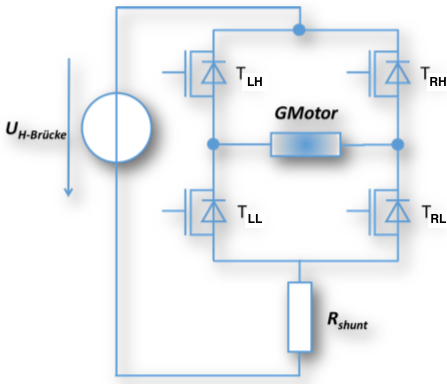
\includegraphics[width=1\textwidth]{schaltung_h_bruecke.png}
    \caption{Schaltung H-Brücke}
    \label{fig:Schaltung H-Bridge}
\end{figure}

Um den Strom positiv, also von links nach rechts, fließen zu lassen,
müssen die MOSFETS $T_{LH}$ und $T_{RL}$ angesteuert werden.\\

Wenn diese beiden besagten Transistoren ausgeschaltet werden, treibt die Energie im
Magnetfeld der Spule den Strom weiter. Dadurch fließt der Motorstrom $I_M$
durch die parasitären Bodydioden der Transistoren $T_{LL}$ und $T_{RH}$.\\

Dieser Strom kann indirekt durch die Spannung die über den Messwiderstand
$R_{Shunt}$ gemessen werden.\\

Soll der Motor in die entgegengesetzte Richtung betrieben werden, müssen
die MOSFETS $T_{RH}$ und $T_{LL}$ angesteuert werden.\\

Dadurch gibt es insgesamt 4 Zustände. Links-Rechts-Lauf Transistoren an oder
ausgeschaltet und Rechts-Links-Lauf Transistoren an oder ausgeschaltet.\\

Um die H-Brücke zu betreiben wird eine Steuerung benötigt. Die Steuerung
benötigt als Eingänge den Sollstrom $I_{soll}$, den momentanen Strom
$I_{ist}$ und die Eingangspannung. Als Ausgänge besitzt die Steuerung die
gepulste Motorspannung.\\

Die 4 Maschengleichung der 4 Zustände lauten wie folgt, wenn der
Drain-Source Widerstand vernachlässigt wird.\\

Link-Rechts-Lauf:

\begin{equation} \label{eq411}
    \begin{split}
        0 &= U_H - R \cdot i_M - L \cdot \dot{i_M} - k_e \cdot \omega - R_{Shunt} \cdot i_M\\
        0 &= U_H + 2 U_D + R \cdot i_M + L \cdot \dot{i_M} + k_e \cdot \omega + R_{Shunt} \cdot i_M
    \end{split}
\end{equation}

Rechts-Links-Lauf:

\begin{equation} \label{eq411}
    \begin{split}
        0 &= U_H + R \cdot i_M + L \cdot \dot{i_M} + k_e \cdot \omega - R_{Shunt} \cdot i_M\\
        0 &= U_H + 2 U_D - R \cdot i_M - L \cdot \dot{i_M} - k_e \cdot \omega + R_{Shunt} \cdot i_M
    \end{split}
\end{equation}


% 2.6
% 1. Fall: AN
%     U_H = U_T_LH + U_Motor + U_T_RL + U_R_shunt

%     U_H = R_LH * I_m + (R_shunt * I_m)  

% 2. Fall: Aus
%     0 = U_H + U_D + U_Motor + U_D + U_shunt